\chapter{Approccio basato su reti prototipiche}

\section{Motivazione: il problema delle classi non viste}
I risultati presentati nel Capitolo~\ref{ch:risultati} hanno mostrato come il micro-drop, ossia la rimozione di intere classi dal training set, produca una degradazione significativa delle prestazioni di classificazione, 
a differenza del macro-drop, il cui impatto è risultato trascurabile su entrambi i dataset considerati. 
Un classificatore standard, tuttavia, non è in grado di riconoscere classi mai osservate durante l'addestramento: la soluzione più diretta con gli approcci tradizionali sarebbe un riaddestramento completo ogni volta che 
emerge una nuova classe da riconoscere, con un costo computazionale spesso proibitivo.

Il \emph{few-shot learning} affronta questo problema proponendo modelli in grado di generalizzare a nuove classi a partire da un numero molto ridotto di esempi, 
senza richiedere un nuovo addestramento della rete. In questo capitolo viene adottato l'approccio delle reti prototipiche, 
che si presta naturalmente a questo scenario grazie alla sua semplicità concettuale e all'assenza di parametri aggiuntivi da apprendere per integrare nuove classi.

\section{Reti prototipiche: principio di funzionamento}
Le reti prototipiche, introdotte da Snell et al.~\cite{snell2017prototypical}, proiettano le immagini in uno spazio di embedding $f_\phi: \mathbb{R}^D \rightarrow \mathbb{R}^M$ 
in cui gli esempi di ciascuna classe $k$ si concentrano attorno a un punto rappresentativo, detto \emph{prototipo}, 
calcolato come media degli embedding del relativo support set $S_k$:
\begin{equation}
    c_k = \frac{1}{|S_k|} \sum_{x \in S_k} f_\phi(x).
\end{equation}
La classificazione di un nuovo esempio $x$ avviene calcolando la distanza (euclidea al quadrato, nella formulazione originale) tra il suo embedding $f_\phi(x)$ e ciascun prototipo $c_k$, assegnando la classe corrispondente secondo la distribuzione softmax sulle distanze:
\begin{equation}
    p_\phi(y=k \mid x) = \frac{\exp(-\|f_\phi(x) - c_k\|^2)}{\sum_{k'} \exp(-\|f_\phi(x) - c_{k'}\|^2)}.
\end{equation}
Questo approccio rende semplice il funzionamento few-shot: è sufficiente disporre di un piccolo numero di esempi (\emph{shot}) per costruire il prototipo di una nuova classe, senza la necessità di riaddestrare l'intero modello.

A differenza della formulazione originale, in cui l'estrattore $f_\phi$ viene addestrato in modo episodico, in questo lavoro i prototipi sono costruiti sulle feature di una rete addestrata con cross-entropy e mantenuta congelata: il modello adottato è quindi un classificatore a prototipi ispirato alle reti prototipiche.

\section{Setup e campionamento}
La valutazione del modello prototipico è stata condotta secondo lo scenario \emph{Generalized Few-Shot}: 
per ciascuna configurazione di micro-drop del Capitolo~\ref{ch:risultati}, i prototipi vengono costruiti sia per le classi note (dall'intero training set) sia per le classi escluse (a partire da $5$ immagini di supporto per classe), 
e la classificazione avviene sul test set completo, il quale comprende entrambe le categorie di classi. 
Questo scenario è stato preferito a una valutazione few-shot ristretta alle sole classi non viste poiché si collega direttamente al problema individuato nel Capitolo~\ref{ch:risultati}: 
verificare se il recupero delle classi mancanti tramite pochi esempi comprometta le prestazioni sulle classi già apprese.

Come estrattore di feature è stato riutilizzato, mantenendone i pesi congelati\footnote{I pesi del modello preso in considerazione non vengono aggiornati. La rete è impiegata per il calcolo degli embedding delle immagini, successivamente utilizzati per costruire i prototipi delle classi.},
il modello già addestrato nel Capitolo~\ref{ch:risultati} per ciascuna architettura e percentuale di micro-drop, 
evitando così un nuovo addestramento e mantenendo la coerenza tra i due esperimenti.

Per il dataset Oxford-IIIT Pet la valutazione è stata ripetuta $30$ volte per ciascuna configurazione, con campionamento casuale del support set a ogni episodio, 
riportando media e deviazione standard sulle metriche. Per CIFAR-100, a causa di vincoli di tempo e di risorse di calcolo, 
la valutazione è stata condotta su un singolo episodio; tale limite è stato tenuto in considerazione nell'interpretazione dei risultati riportati in Sezione~\ref{sec:proto-risultati-discussione}.
Per entrambi i dataset il campionamento del support set è governato dal seed \texttt{777}; per CIFAR-100 il modello riutilizzato è quello addestrato con seed \texttt{42}, l'unico disponibile (Sezione~\ref{sec:cifar100}).

\section{Risultati ottenuti e discussione}
\label{sec:proto-risultati-discussione}

Come mostrato in Figura~\ref{fig:pet-proto-micro} e in Tabella~\ref{tab:proto-pet}, su Oxford-IIIT Pet EfficientNet mantiene le prestazioni più elevate sulle classi note e, in media sui tre livelli di drop, anche su quelle recuperate tramite few-shot, confermando il pattern di robustezza già osservato nel Capitolo~\ref{ch:risultati}. Le classi recuperate mostrano un'Accuracy sistematicamente più bassa rispetto a quelle note (tra circa $20$ e $33$ punti percentuali di differenza) e una variabilità marcatamente maggiore tra gli episodi, coerente con l'aspettativa che $5$ soli esempi di supporto per classe producano prototipi meno stabili rispetto a quelli costruiti sull'intero training set.

\begin{figure}[htbp]
    \centering
    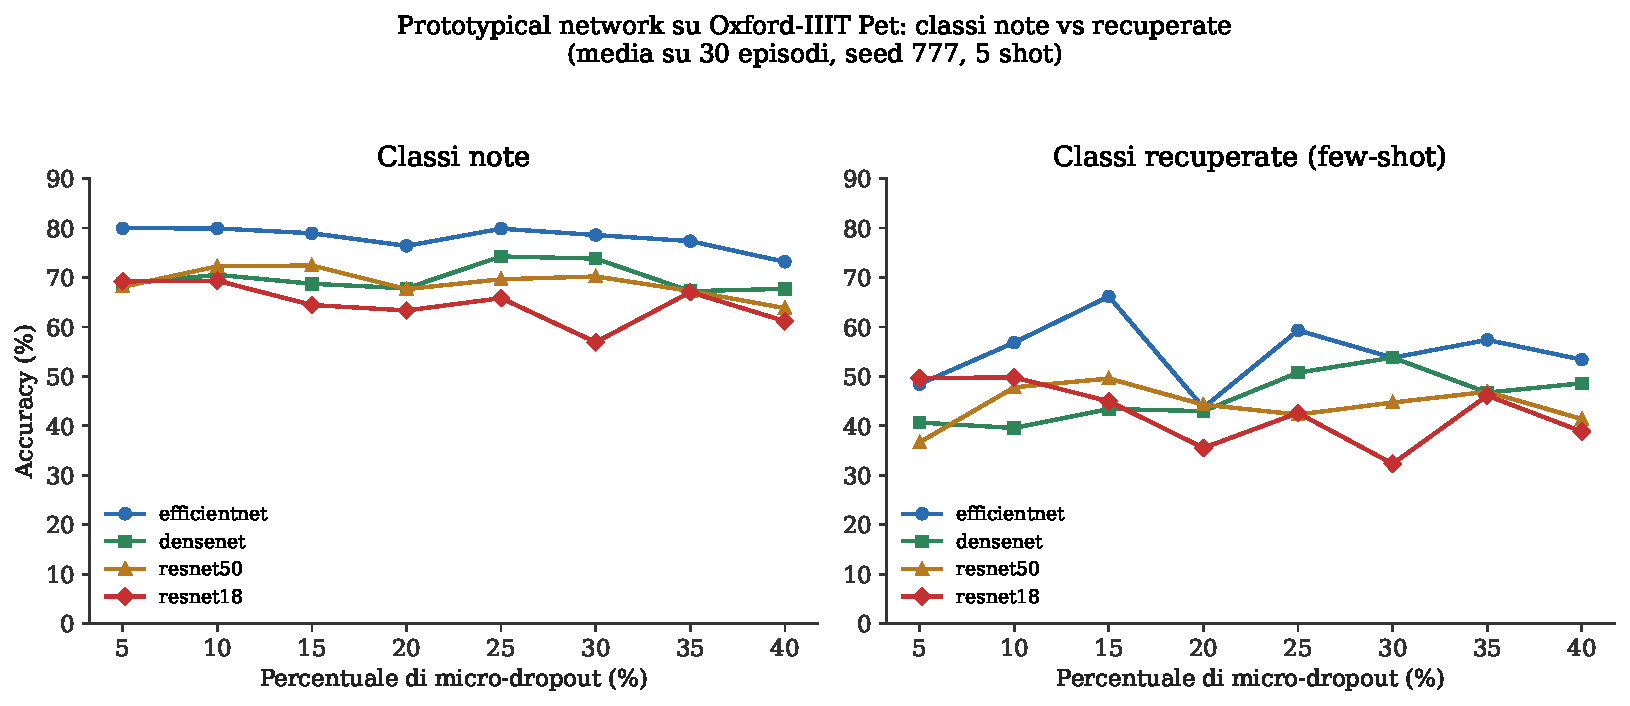
\includegraphics[width=\textwidth]{figures/pet_proto_micro.pdf}
    \caption{Accuracy del modello prototipico su Oxford-IIIT Pet, separata tra classi note (sinistra) e classi recuperate tramite few-shot (destra), al variare della percentuale di micro-drop. Media su 30 episodi, seed 777, 5 shot per classe.}
    \label{fig:pet-proto-micro}
\end{figure}

\begin{table}[!htb]
    \centering
    \small
    \caption{Accuracy (\%) sulle classi note e sulle classi recuperate tramite few-shot, per le quattro architetture sul dataset Oxford-IIIT Pet. Media $\pm$ deviazione standard su 30 episodi.}
    \label{tab:proto-pet}
    \begin{tabular}{llccc}
        \toprule
        \textbf{Modello} & \textbf{Drop \%} & \textbf{Acc. Note} & \textbf{Acc. Ignote} & \textbf{Classi escluse} \\
        \midrule
        \multirow{3}{*}{EfficientNet} & 5  & $79.93 \pm 1.27$ & $48.44 \pm 6.43$  & 1 \\
                                       & 20 & $76.37 \pm 1.09$ & $43.67 \pm 4.43$  & 4 \\
                                       & 40 & $73.15 \pm 1.45$ & $53.37 \pm 4.08$  & 9 \\
        \midrule
        \multirow{3}{*}{DenseNet}     & 5  & $68.66 \pm 1.35$ & $40.67 \pm 8.32$  & 1 \\ 
                                       & 20 & $67.79 \pm 1.37$ & $42.97 \pm 5.40$  & 4 \\
                                       & 40 & $67.69 \pm 1.26$ & $48.60 \pm 3.24$  & 9 \\
        \midrule
        \multirow{3}{*}{ResNet50}     & 5  & $68.11 \pm 1.55$ & $36.67 \pm 10.78$ & 1 \\
                                       & 20 & $67.63 \pm 1.33$ & $44.28 \pm 5.12$  & 4 \\
                                       & 40 & $63.78 \pm 1.59$ & $41.38 \pm 2.60$  & 9 \\
        \midrule
        \multirow{3}{*}{ResNet18}     & 5  & $69.18 \pm 1.14$ & $49.67 \pm 9.12$  & 1 \\
                                       & 20 & $63.32 \pm 1.22$ & $35.53 \pm 4.21$  & 4 \\
                                       & 40 & $61.15 \pm 1.57$ & $38.85 \pm 4.40$  & 9 \\
        \bottomrule
    \end{tabular}
\end{table}

Confrontando questi risultati con la baseline del Capitolo~\ref{ch:risultati} (senza recupero few-shot), l'introduzione del modello prototipico comporta generalmente un peggioramento moderato delle prestazioni sulle classi note per tutte e quattro le architetture, con perdite comprese tra circa $1$ e $13$ punti percentuali a seconda del modello e della percentuale di drop. Questo suggerisce che l'aggiunta dei prototipi delle classi non viste introduce un certo grado di interferenza nello spazio degli embedding condiviso, più marcata per ResNet50 e minore per EfficientNet.

\FloatBarrier

I risultati su CIFAR-100 (Tabella~\ref{tab:proto-cifar}), pur limitati a un singolo episodio, mostrano un divario più contenuto tra classi note e classi recuperate rispetto a quanto rilevato su Oxford-IIIT Pet. Sebbene tale confronto debba tenere conto della diversa metrica impiegata nei report (Macro F1-score per CIFAR-100 rispetto all'Accuracy per Oxford-IIIT Pet), una possibile spiegazione è che la minore separazione tra i prototipi su CIFAR-100 ($100$ classi totali contro $37$) renda la distanza mediamente inferiore e quindi lo spazio decisionale più uniforme tra classi note e classi recuperate.

\begin{table}[!htb]
    \centering
    \small
    \caption{Macro F1-score (\%) sulle classi note e sulle classi recuperate tramite few-shot, per EfficientNet e ResNet50 sul dataset CIFAR-100 (singolo episodio, seed 777).}
    \label{tab:proto-cifar}
    \begin{tabular}{llcc}
        \toprule
        \textbf{Modello} & \textbf{Drop \%} & \textbf{F1 Note} & \textbf{F1 Ignote} \\
        \midrule
        \multirow{3}{*}{EfficientNet} & 5  & 68.35 & 66.84 \\
                                       & 20 & 65.17 & 61.80 \\
                                       & 40 & 59.60 & 51.04 \\
        \midrule
        \multirow{3}{*}{ResNet50}     & 5  & 60.32 & 57.33 \\
                                       & 20 & 57.04 & 50.65 \\
                                       & 40 & 54.32 & 42.82 \\
        \bottomrule
    \end{tabular}
\end{table}

In sintesi, il modello prototipico si conferma una soluzione efficace per recuperare parzialmente la capacità di riconoscere classi escluse dal training, sebbene con prestazioni inferiori rispetto a quelle ottenute sulle classi apprese in modo completo e con un costo moderato sulle prestazioni delle classi note, più evidente su Pet che su CIFAR-100.
